\newpage
%\chapter{Descripción} \label{cap:Herramienta SLAMTestBed}
\chapter{Herramienta SLAMTestBed} \label{cap:Herramienta SLAMTestBed} %chapter 4
\setcounter{section}{4}
En este capítulo se detallará el diseño de la herramienta SLAMTestBed, una herramienta diseñada para comparar algoritmos SLAM. El diseño de algoritmos SLAM es todavía una disciplina abierta en periodo de expansión. En la navegación autónoma de robots y drones es donde mayor importancia alcanza la utilización de los algoritmos SLAM. Pero algoritmos hay muchos y se necesitan herramientas que nos permitan medir la bondad de cada algoritmo.
Comenzaremos explicando el diseño desde un punto de vista de Caja Negra, explicando las entradas y las salidas. Se continuará con la explicación del diseño en Caja Blanca y se finalizará explicando cada uno de los componentes principales de la herramienta , como los distintos módulos que permiten calcular el Registro Espacial ( Escala, Traslación y Rotación) y el Registro Temporal (interpolación de frecuencias y cálculo de Offset o Desplazamiento Temporal)

\subsection{Diseño de Caja Negra}

En esta sección no entraremos en los detalles de la implementación de la herramienta SLAMTestBed, si no que lo trataremos como una \textit{caja negra}.
De un lado tendremos las entradas al sistema, que serán 2 datasets.
Una vez procesados los 2 datasets por la caja negra, obtendremos a la salida, las transformaciones estimadas por la herramienta, junto con un dataset estimado que utilizaremos para medir el error cometido en las estimaciones.


\begin{figure}[H]
\begin{center}
\subfigure[]{\label{fig:Open File}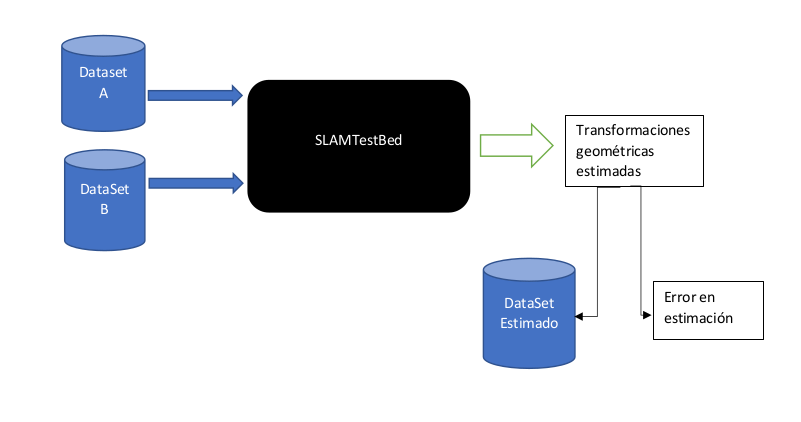
\includegraphics[height=6.0cm,width=12.0cm]{img/cap5/Esquema_TFM_CajaNegra.png}}
\hspace{0.5cm}
%\subfigure[]{\label{fig:LG_hombot}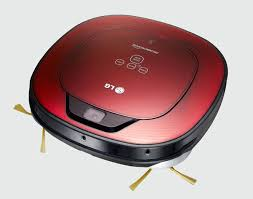
\includegraphics[height=6.0cm]{img/cap2/LG_hombot.jpg}}
\end{center}
%\caption{Robot Dyson 360 Eye (a) Robot Roomba 966 (b) Robot Hombot de LG (c).}
\caption{ En la imagen superior, el diseño de Caja Negra de la herramienta SLAMTestBed }
\end{figure}

\subsection{Diseño de caja Blanca}
En esta sección explicaremos con más detalle la implementación de la herramienta SLAMTestBed.
Las entradas y salidas del sistema serán las mismas que las explicadas en la sección anterior (Diseño de Caja Negra).

\textbf{La explicación del algoritmo:}
En este apartado explicaremos los pasos seguidos para hacer los cálculos que nos permitiran estimar las transformaciones requeridas para pasar de un dataset A a otro dataSet B. 
Las principales funciones o módulos de los que constará la herramienta será:
\begin{description}
\item [Cálculo de PCA]: Nos permitirá reducir el dataset a  sus componentes principales.
\item [Estimación de Escala]: Estimará la diferencia de escala entre los dos datasets.
\item [Estimación de Offset]: Con este módulo podremos hallar la diferencia entre marcas de tiempos de los 2 datasets.
\item [Interpolación para igualar frecuencias de muestreo]: Con la interpolación podremos igualar en frecuencias los dos datasets.
\item [Operaciones de Registro para estimar la Rotación y Traslación]: Permitirá estimar las traslación y rotación necesarias para pasar de un datasetA a un datasetB.
\end{description}


\begin{figure}[H]
\begin{center}
\subfigure[]{\label{fig:Open File}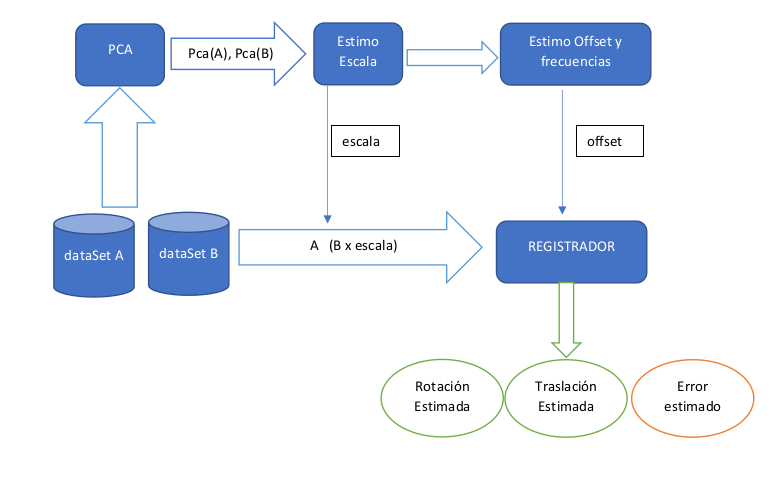
\includegraphics[height=8.0cm,width=12.0cm]{img/cap5/EsquemaTFM_CajaBlanca_Transformaciones.png}}
\hspace{0.5cm}
%\subfigure[]{\label{fig:LG_hombot}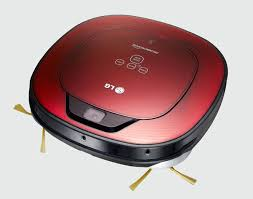
\includegraphics[height=6.0cm]{img/cap2/LG_hombot.jpg}}
\end{center}
%\caption{Robot Dyson 360 Eye (a) Robot Roomba 966 (b) Robot Hombot de LG (c).}
\caption{ En la imagen superior, el diseño de Caja Blanca de la herramienta SLAMTestBed }
\end{figure}

Básicamente el flujo de datos que sigue la imagen superior es el siguiente:

Se calculará la descomponsición en componentes principales (PCA) para cada dataset, con estos nuevos datasets, calularemos la escala. Posteriormente estimaremos el offset de tiempo entre los dos datasets y unificaremos las frecuencias. 

Con los datos dataSetApca y dataSetBpca estimaremos el offset de tiempo que exista entre las 2 secuencias de datos o datasets. Posteriormente corregiremos el offset en el dataset B, para ello sumaremos el valor del offset a los valores de tiempo del datasetB. Una vez tengamos calculado el offset, unificaremos las frecuencias de los 2 datasets mediante interpolación. Cuando tengamos unificada la frecuencia para los dos datasets, obtendremos de nuevo PCA de cada dataset y por último obtendremos la escala.
Posteriormente estimaremos  la transformaciones de rotación y traslación para pasar del datasetA al datasetB. Aplicaremos dichas transformaciones sobre el datasetA, que como resultado nos dará un nuevo dataset, el dataset Estimado que pintaremos en pantalla de color rojo.
Más adelante se explicarán con más detalle cada uno de estos módulos.


\subsection{Estimador PCA y Cálculo de Escala}

	Con el módulo PCA obtendremos las componentes principales de un dataset, generando un nuevo dataset.

	A partir de los nuevos datasets generados podremos calcular la escala y la diferencia de tiempos entre los 2 datasets.

	Se implementan 2 métodos de cálculo de PCA, el segundo utilizando el método SVD (utilizando la librería Eigen), que describiremos acontinuación.

	\begin{lstlisting}
		
		mX = media (dataset.x)
		mY = media (dataset.y)
		mZ = media (dataset.z)

		restar la media a cada componente x, y z

		dataset2.x = dataset.x - mX
		dataset2.y = dataset.y - mY
		dataset2.z = dataset.z - mZ

		cov = obtenerMatrizCovarianza(dataset2)
		svd = CalularSVD(cov )
		pca =  Matriz V del resultado svd
		datasetResultado = dataset * Matriz (svd.V)

	\end{lstlisting}

    En cuanto al cálculo de la Escala, nos permitirá calcular la diferencia de escala entre los dos datasets, y así al tener los datasets en la misma escala, ya tendríamos el primer paso del registro espacial. El algoritmo utilizado estará basado en la utilización de los valores singulares de cada datasets.
        
	\begin{lstlisting}
		S1 = svd(dataSet1).valoresSingulares
		S2 = svd(dataSet2).valoresSingulares
		scalaX = S2(0)  / S1(0)
		scalaY = S2(1)  / S1(1)
		scalaZ = S2(2)  / S1(2)
	\end{lstlisting}

\subsection{Registro Espacial}

Con el registro espacial conseguiremos estimar la matriz de rotación y traslación para aplicarlas sobre el segundo dataset, intentando conseguir la operación de registro de los 2 datasets.



\begin{description}
	\item [Hallar la matrices de rotación y traslación] .

		El algoritmo para esta funcionalidad sería el siguiente:
        \begin{lstlisting}
        - Hallar los centroides de las coordenadas X,Y,Z de cada dataset
        	centA = centroides (A)
        	centB = centroides (B)
        

        - Restar los centroides a sus respectivas matrices
          	A= A-centA
          	B= B-centB
        
        - Calcular el producto de las matrices
        	H = A.traspuesta * B

        - Obtener valores singulares de la matriz H
        	S,U,V = svd(H)
        
        - Obtener la matriz de Rotacion
          	R = V*U.traspuesta

        - Obtener la matriz de Traslacion
        	t= -R * centA + centB;  
        \end{lstlisting}

	\item[Transformar un dataset en otro aplicando las matrices de Rotación y Traslación previamenete estimadas]

		Este método tomará un dataset , lo multiplicará por la matriz de rotación y le sumará la matriz de traslación.

	\item[Transformar los cuaternios aplicando la matriz Rotación.]

		Con este método conseguimos transformar los cuarternios del dataSetA al dataSetB.
		Para ello convertiremos la matriz de rotación en un cuaternio que llamaremos "q".
		Por último multiplicaremos cara quaternio p de la siguiente forma.
		  q * p * q.inverso 

	\item[Estimar las matrices de rotación y traslación mediante la técnica de RANSAC.]

		Estimaremos las matrices de Rotación y Traslación utilizando los datos de los 2 datasets.

		El algoritmo seguido ha sido el siguiente:
            \begin{lstlisting}
            	Mientras no alcancemos el numero maximo de iteraciones hacer
            			Seleccionar n inliers
            			Estimar una primera matriz de Rotacion , Traslacion
            			aplicar transformacion sobre un subconjunto de puntos No Inliers
            			Si el error < threshhold
            				aniadir cadidato a inliers
            			medir el error tras aplicar transformaciones sobre inliers y no inliers
            			seleccionar menor error
            			incrementar iteraccion
            	Devolveremos las matrices de Rotacion Traslacion que menor error hayan dado
            \end{lstlisting}
	        

    \end{description}


\subsection{Estimador Offset}

	Con este módulo podremos calcular el offset o desplazamiento en el tiempo entre los 2 datasets.
	El método principal utilizado para calcular el offset se realiza mediante el calculo de la Correlación Cruzada.
	Para ello previamente , calcularemos la distancia al origen para cada punto 3D de los 2 datasets.
	Para un punto 3d (x,y,z), la distancia 3d se calculará 
	\begin{math}
	\sqrt{(x-0)^2 +(y-0)^2+(z-0)^2}
	\end{math}
	una vez calculadas las distancias , aplicaremos el siguiente algoritmo de calculo de correlación cruzada

Este módulo se encarga de estimar el offset o diferencia de tiempo entre los dos datasets. Es el algoritmo más pesado ya que incluye múltiples cálculos para interpolar y calcular 
la correlación cruzada entre los dos datasets.

Este algoritmo será iterativo y utilizaremos un dataset como base de tiempo fijo y otro dataset B que se deslizará en el tiempo desde -T hasta +T . El datasetB se irá 
deslizando en pequeños espacios de tiempo o steps en cada iteración. Para cada step calcularemos la correlación cruzada entre el dataset deslizante y el dataset original (que se 
mantiene fijo en el tiempo). Para un step determinado la correlación debe ser máxima entre los 2 datasets y una vez hallada la correlación máxima, el step de esa iteración nos 
indicará el offset. Como hemos comentado, moveremos el datasetB hasta llegar a -T y por cada iteración iremos deslizando en el tiempo el datasetB un incremento de tiempo step , hasta el final del bucle que terminaremos de deslizar datasetB hasta llegar a un tiempo +T. En cada iteracción calcularemos la interpolación en los puntos que coincidan que esten dentro de los rangos temporales de los dos datasets. Una vez interpolados los puntos comunes de las 2 series tendremos 2 series nuevas, Para las cuales calcularemos la correlación cruzada aplicando el algoritmo típico para 2 series temporales. Pero antes, y como cada serie temporal tiene 3 coordenadas (x,y,z para cada punto 3d), debemos transformar estas 3 coordenadas en un sólo valor para cada punto 3D de cada serie, para ello calcularemos la distancia al origen de todo punto 3D, y por tanto la correlación cruzada se calculará sobre los 2 datasets convertidos a distancias al origen de coordenadas.

\begin{figure}[H]
\begin{center}
\subfigure[]{\label{fig:opciones de View}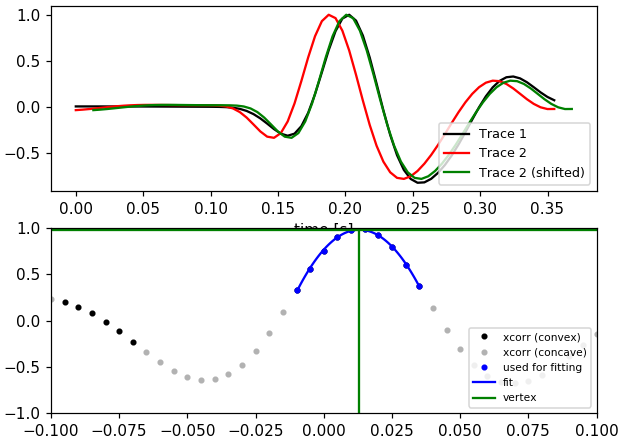
\includegraphics[height=8.0cm,width=12.0cm]{img/cap5/correlacionCruzada.png}}
\hspace{0.5cm}

\end{center}

\caption{Gráfico que muestra el desfase del offset entre dos series temporales y el resultado de la correlación cruzada.}
\end{figure}
	                                
	\begin{lstlisting}
	dataA = CalcularDistancia( dataSetA)
	dataB = CalcularDistancia( dataSetB)
	mA = CalcularMedia(dataA)
	mB = CalularMedia(dataB)

	Para cada fila

   		sx = dataA(i) - mA

   		sy = dataB(i) - mB

   	denom = sqrt(sx*sy);
   	step = 0.01
   	Desde i=-T hasta i = T
   		Si ( dataB.t < dataB.t )
			j=j+1
    		continuar

    	sino si (dataB.t > dataA.t)
    		i=i+1
    		continuar

    	sino si (dataB.t == dataA.t)
    		sxy=(dataA -mA) * (dataB-mB)
        	i++
        	j++


   

   r = (sxy) / denom;

   r= fabs(r);
    \end{lstlisting}



\subsection{Interpolador}

	El módulo de interpolación se utiliza para sincronizar a igual frecuencia 2 datasets.
	Entre las distintas funciones , permite sincronización a la frecuencia mayor de los 2 datasets, sincronización a la frecuencia menor de los 2 datasets o incluso consigue sincronizar las 2 series a una frecuencia deseada. La interpolación se realiza sobre las secuencias temporales de los 2 datasets, pero tambien se calcula la interpolación para las coordenadas X,Y y Z de cada punto 3D y se realiza tambien interpolación para los quaternios. La función \textit{slerp} de la librería Eigen nos permite calcular la interpolación entre quaternios. La función slerp recibe como parámetro una marca de tiempo y un quaternio.

\subsection{Cálculo de Estadísticas}

Para medir el erro cometido entre el dataset Groundtruth y el dataset Estimado utilizaremos el módulo de Cálculo de Estadísticas.
Este módulo permite calcular el Error Cuadrático Medio (Root Mean Square Error) entre 2 datasets.
Cuanto menor sea el RMSE , mejor será el dataset Estimado.
También nos permite hallar la media, mediana , máximo y mínimo valor de un dataset.


\subsection{GUI}

Para la herramienta SLAMTestBed tambien se ha diseñado y creado un Interfaz de Usuario Gráfico (GUI) que permita pintar los puntos 3D de cada dataset en pantalla así como invocar comandos (a través de clicks de ratón) para ejecutar los distintos módulos que contiene la herramienta SLAMTestBed.
Nos permitirá medir la exactitud de los resultados de la aplicación de un algoritmo con los resultados de otro algoritmo o comparar varios resultados de un mismo algoritmo en el que se han aplicado distintos parámetros de ejecución.
Este interfáz gráfico de usuario de 3 dimensiones ha sido desarrollado en C++ con el entorno QT y la librería Eigen. La libería Eigen es una librería Open Source realizada en C++, para cálculos de Álgebra lineal, operaciones con Matrices y vectores, Transformaciones Geométricas. 

La aplicación sofware muestra al usuario un interfaz gráfico que permite:
Leer un archivo de datos con puntos 3D y mostrarlo en pantalla como una nube de puntos 3D. Este archivo podriamos denominarlo groundTruth.
Con el ratón podremos girar en 3 dimensiones la nube de puntos, acercarnos a el (Zoom in) o alejarnos (Zoom Out),
tambien permite leer un segundo conjunto de puntos 3D y estimar las transformaciones ( rotaciones , traslaciones, escala etc)  necesarias para pasar desde el conjunto de datos ground truth hasta este segundo conjunto de datos. El conjunto de datos resultante tras aplicar las estimaciones será visulalizado en pantalla como otra nube de puntos 3D

\begin{figure}[H]
\begin{center}
\subfigure[]{\label{fig:Transformaciones versus Estimaciones}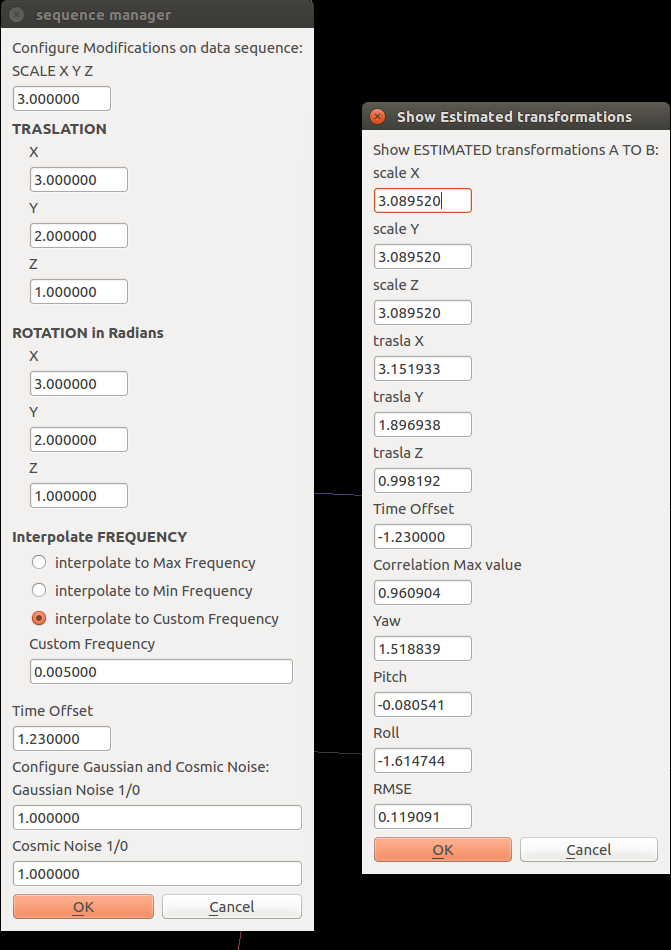
\includegraphics[height=12.0cm,width=8.0cm]{img/cap5/showTransformationsEstimated.png}}
\hspace{0.5cm}
\end{center}
\caption{Transformaciones realizadas frente Transformaciones estimadas }
\end{figure}


\begin{figure}[H]
\begin{center}
\subfigure[]{\label{fig:opciones de View}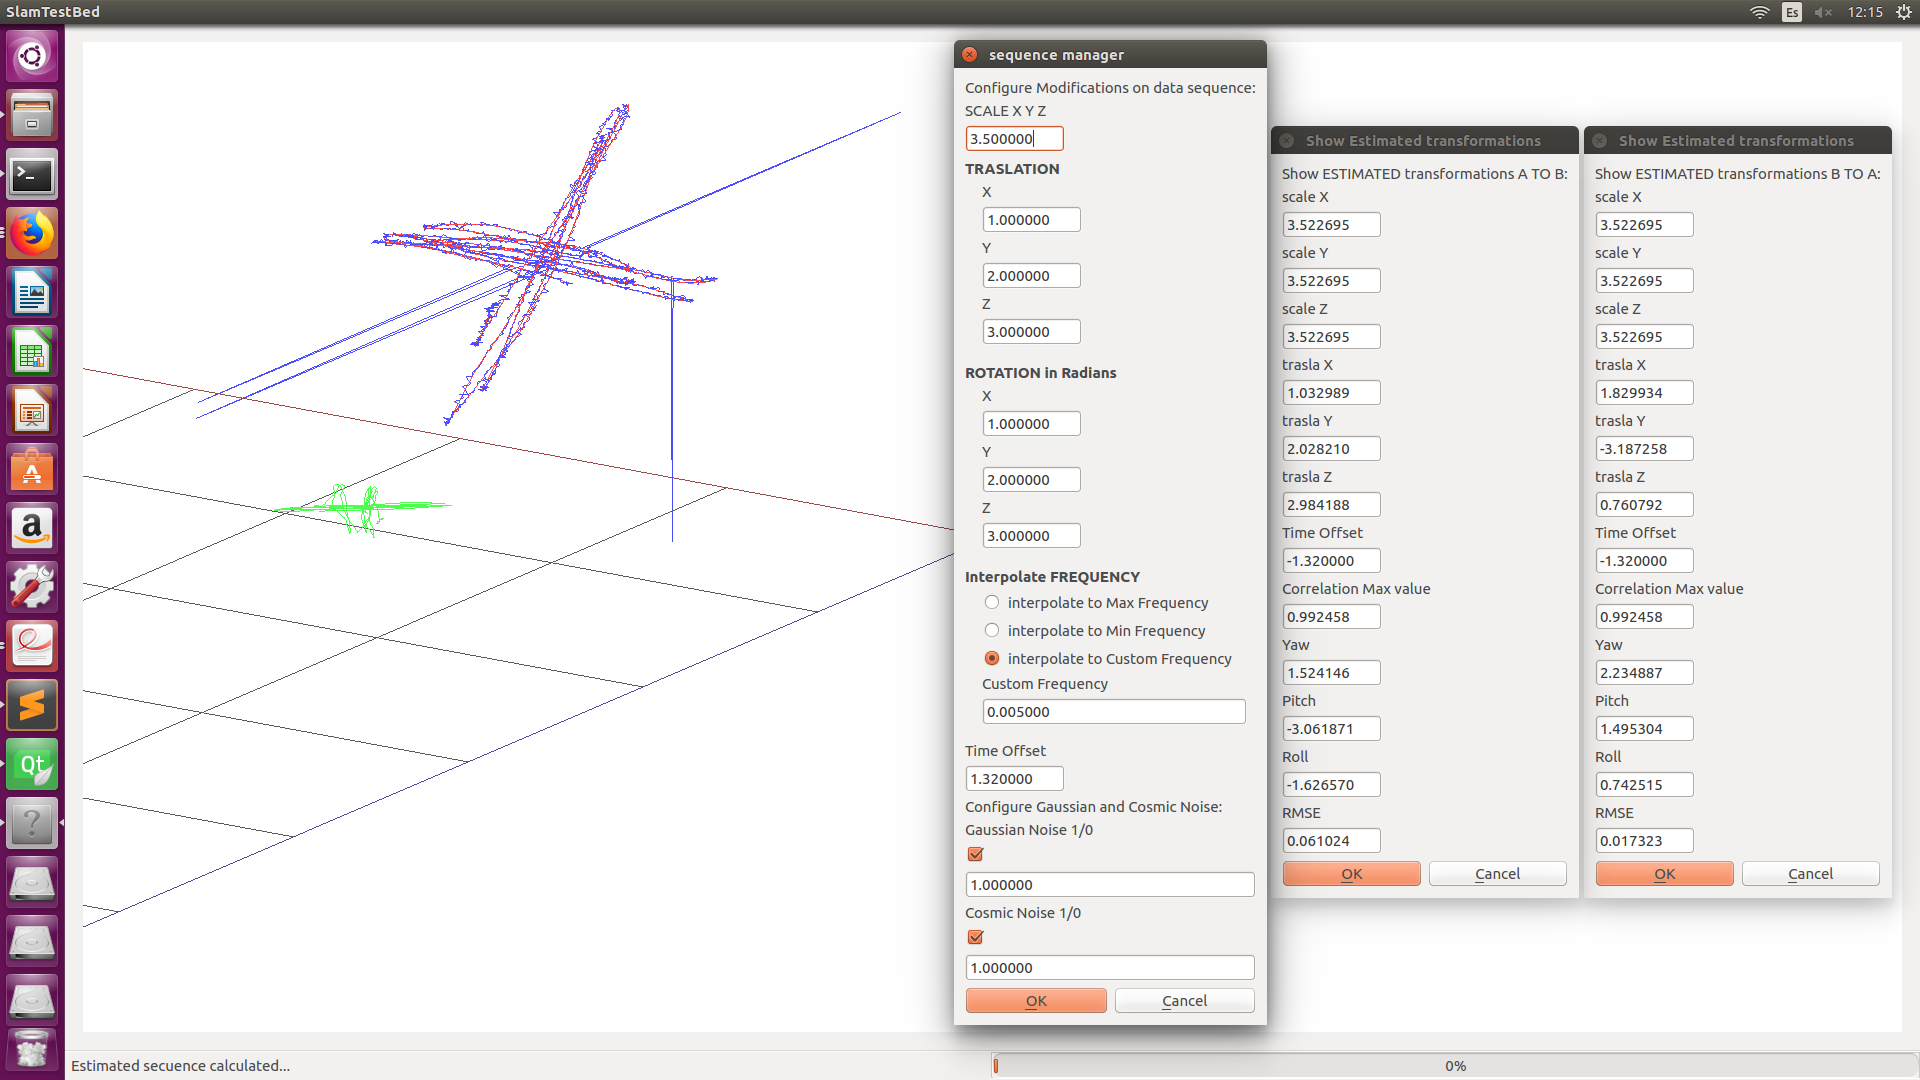
\includegraphics[height=10.0cm,width=15.0cm]{img/cap6/Escala_Trasla_Rota_Offset_Gauss_CosmicNoise_abba.png}}
\hspace{0.5cm}

\end{center}

\caption{Gráfico que muestra los resultados de la estimación de un cambio de escala y traslación .}
\end{figure}

En la pantalla gráfica podremos ver los 3 datasets. Los puntos 3D del dataset groundtrouth se pintarán en color verde, los puntos del dataset a evaluar o dataset transformado serán de color azul , y por último en color rojo estarán los puntos 3D del dataset estimado.


\clearpage

